\documentclass[11pt,a4paper]{article}

% ─── Packages ────────────────────────────────────────────────────────────
\usepackage[utf8]{inputenc}
\usepackage[T1]{fontenc}
\usepackage{amsmath,amssymb,bm}
\usepackage{graphicx}
\usepackage{booktabs}
\usepackage{siunitx}
\usepackage[margin=2.5cm]{geometry}
\usepackage{hyperref}
\usepackage{cleveref}
\usepackage{caption,subcaption}
\usepackage{xcolor}
\usepackage{enumitem}
\usepackage{mathtools}

% ─── Custom commands ─────────────────────────────────────────────────────
\newcommand{\alphag}{\alpha_{\mathrm{g}}}
\newcommand{\Vz}{V_z}
\newcommand{\ERMS}{E_{\mathrm{RMS}}}
\newcommand{\dd}{\mathrm{d}}

% ─── Title ───────────────────────────────────────────────────────────────
\title{%
  Accuracy of Rise Velocity Estimation from Lagrangian Particle Tracking
  Data: \\[4pt]
  A Comparative Analysis of Scattered and Interpolated Approaches}
\author{}
\date{}

\begin{document}
\maketitle

% =========================================================================
\begin{abstract}
In Lagrangian particle tracking (LPT) simulations of multiphase flows, field
quantities such as gas volume fraction and velocity are carried by discrete
particles that move to irregular, scattered positions over time.  A
fundamental question is how accurately one can recover integral flow
diagnostics---in particular the bubble rise velocity---from these scattered
Lagrangian data, compared with the reference solution on the original
Eulerian grid.  This document presents a systematic numerical analysis of
rise velocity estimation for a two-dimensional axisymmetric rising bubble at
$\mathrm{Re}=100$, $\mathrm{Bo}=100$.  Two definitions of rise velocity
(centroid-based and volume-averaged) are evaluated under four interpolation
scheme combinations (linear/cubic for velocity and gas fraction) and two
data representations (raw scattered particles versus re-interpolation onto a
fixed Eulerian grid).  The analysis reveals that: (i)~the centroid-based
rise velocity is consistently more accurate than the volume-averaged
approach; (ii)~re-interpolating scattered data onto a fixed grid dramatically
improves centroid-based estimates while offering limited benefit for the
volume-averaged method; and (iii)~the dominant source of error is the
velocity field interpolation rather than the gas fraction field.
\end{abstract}

% =========================================================================
\section{Introduction}\label{sec:intro}

Consider a gas bubble rising through a quiescent liquid, a canonical problem
in multiphase fluid dynamics.  When solving the governing equations on a
fixed Eulerian grid, the gas volume fraction field
$\alphag(\bm{x},t)$ and the velocity field $\bm{V}(\bm{x},t)$ are
naturally available at every grid node.  Computing integral diagnostics such
as the bubble rise velocity from these gridded fields is straightforward.

An alternative Lagrangian viewpoint tracks a cloud of neutrally buoyant
marker particles that are initially seeded at every Eulerian grid node,
giving a total of $n_r \times n_z$ particles (where $n_r$ and $n_z$ denote
the number of grid points in the radial and axial directions, respectively).
Each particle carries the local gas fraction $\alphag$ and axial velocity
$\Vz$ that are interpolated from the Eulerian field to the particle
position at every time step.  Because the particles are advected by the
flow, their positions become irregularly distributed (scattered) over time.

While this Lagrangian representation is advantageous for data-driven modal
decomposition methods such as Proper Orthogonal Decomposition (POD) and
Dynamic Mode Decomposition (DMD), it introduces interpolation errors and
raises the question: \emph{how accurately can the bubble rise velocity be
recovered from scattered Lagrangian particle data?}

Three principal sources of error are identified:
\begin{enumerate}[label=(\roman*)]
  \item \textbf{Interpolation scheme:} During particle tracking, the
        Eulerian fields are interpolated to each particle position using
        either linear or cubic interpolation, for both the velocity and gas
        fraction fields independently.
  \item \textbf{Data representation:} The rise velocity can be computed
        either directly from the scattered particle data or after
        re-interpolating the scattered data back onto a fixed Eulerian grid.
  \item \textbf{Rise velocity definition:} Two physically motivated
        definitions are available---centroid-based and volume-averaged---each
        with different sensitivities to field errors.
\end{enumerate}

This document provides a detailed mathematical description of each
approach (\cref{sec:formulation}), describes the numerical setup
(\cref{sec:setup}), and analyses the results (\cref{sec:results}).


% =========================================================================
\section{Mathematical Formulation}\label{sec:formulation}

\subsection{Problem setting}

We consider a two-dimensional axisymmetric domain parameterised by the
radial coordinate $r$ and the axial coordinate $z$.  The Eulerian grid has
$n_r$ points in the $r$-direction and $n_z$ points in the $z$-direction,
forming a structured mesh $\{(r_i, z_j)\}$.  At each time step $t^n$, the
Eulerian solution provides:
\begin{itemize}
  \item $\alphag(r_i,z_j,t^n)$: the gas volume fraction, and
  \item $\Vz(r_i,z_j,t^n)$: the axial (vertical) velocity component.
\end{itemize}

A set of $N_p = n_r \times n_z$ neutrally buoyant Lagrangian particles is
initialised at the Eulerian grid nodes.  At subsequent times, each particle
$p$ has a displaced position $\bm{x}_p(t) = (r_p, z_p)$ and carries scalar
values $\alphag^{(p)}$ and $\Vz^{(p)}$ obtained by interpolating the
Eulerian fields to the particle location.

% ─────────────────────────────────────────────────────────────────────────
\subsection{Interpolation during particle tracking}
\label{sec:interp_tracking}

At each time step of the tracking algorithm, the Eulerian fields
$\alphag(\bm{x},t)$ and $\Vz(\bm{x},t)$ must be evaluated at the
particle position $\bm{x}_p$.  Two interpolation schemes are employed:

\paragraph{Linear interpolation.}
The field value at $\bm{x}_p$ is obtained by bilinear interpolation from
the four surrounding Eulerian grid nodes.  For a scalar field $\phi$:
\begin{equation}\label{eq:bilinear}
  \phi(\bm{x}_p) = \sum_{i=1}^{4} w_i \, \phi(\bm{x}_i)
  ,\qquad
  \sum_{i=1}^{4} w_i = 1,
\end{equation}
where $w_i$ are the standard bilinear weights based on the normalised
distances within the bounding cell.

\paragraph{Cubic interpolation.}
The field is evaluated using a bicubic interpolation stencil involving the
$4\times 4$ surrounding grid nodes, providing higher-order accuracy at the
cost of a wider stencil.

Since the velocity and gas fraction fields can use different interpolation
schemes independently, four combinations arise:
\begin{center}
\begin{tabular}{lcc}
  \toprule
  Case & $\alphag$ interpolation & $\Vz$ interpolation \\
  \midrule
  G-linear / V-linear & Linear & Linear \\
  G-linear / V-cubic  & Linear & Cubic  \\
  G-cubic  / V-linear & Cubic  & Linear \\
  G-cubic  / V-cubic  & Cubic  & Cubic  \\
  \bottomrule
\end{tabular}
\end{center}

% ─────────────────────────────────────────────────────────────────────────
\subsection{Rise velocity definitions}
\label{sec:rise_vel_defs}

Two definitions of the bubble rise velocity are considered.  In an
axisymmetric domain, all integrals below are area-weighted by the radial
coordinate $r$.

\subsubsection{Method~1: Centroid-based rise velocity}
\label{sec:centroid}

The centroid-based rise velocity is obtained by first computing the
$\alphag$-weighted centroid of the bubble in the axial direction, and then
differentiating its position in time.

\paragraph{Step 1: Bubble centroid.}
On the structured Eulerian grid, the axial position of the bubble centroid
at time $t^n$ is defined as
\begin{equation}\label{eq:centroid_euler}
  z_c(t^n) = \frac{%
    \displaystyle\sum_{i=1}^{n_r}\sum_{j=1}^{n_z}
      \alphag(r_i,z_j,t^n)\, z_j
  }{%
    \displaystyle\sum_{i=1}^{n_r}\sum_{j=1}^{n_z}
      \alphag(r_i,z_j,t^n)
  }\,.
\end{equation}
For the scattered Lagrangian data (without re-gridding), the equivalent
expression uses the particle-carried quantities directly:
\begin{equation}\label{eq:centroid_lag}
  z_c(t^n) = \frac{%
    \displaystyle\sum_{p=1}^{N_p} \alphag^{(p)}(t^n)\, z_p(t^n)
  }{%
    \displaystyle\sum_{p=1}^{N_p} \alphag^{(p)}(t^n)
  }\,.
\end{equation}

\paragraph{Step 2: Rise velocity via finite differencing.}
The centroid-based rise velocity is computed as
\begin{equation}\label{eq:vrise_centroid}
  V_{\mathrm{rise}}^{\mathrm{cent}}(t^n)
  = \frac{z_c(t^n) - z_c(t^{n-1})}{t^n - t^{n-1}}
  = \frac{z_c(t^n) - z_c(t^{n-1})}{\Delta t}\,,
\end{equation}
where $\Delta t$ is the time step between snapshots.  This method relies
\emph{solely} on the gas volume fraction field; the velocity field is not
used.  Consequently, any error in $\alphag$ interpolation directly affects
the centroid position and, through finite differencing, the estimated rise
velocity.  This is implemented in the function
\texttt{rise\_velocity\_centroid}, which returns both $z_c(t^n)$ and
$V_{\mathrm{rise}}^{\mathrm{cent}}(t^n)$.

\subsubsection{Method~2: Volume-averaged rise velocity}
\label{sec:vol_avg}

The volume-averaged rise velocity computes the gas-fraction-weighted,
radially-weighted mean of the axial velocity inside the bubble region.

\paragraph{Step 1: Bubble identification.}
The bubble region $\Omega_b$ is defined by a threshold on the gas volume
fraction:
\begin{equation}\label{eq:bubble_mask}
  \Omega_b(t^n) = \bigl\{\, \bm{x} : \alphag(\bm{x},t^n) \geq
    \alpha_{\mathrm{th}} \,\bigr\}\,,
  \qquad \alpha_{\mathrm{th}} = 0.5\,.
\end{equation}

\paragraph{Step 2: Weighted velocity average.}
On the structured Eulerian grid, the volume-averaged rise velocity is
\begin{equation}\label{eq:vrise_volavg}
  V_{\mathrm{rise}}^{\mathrm{vol}}(t^n)
  = \frac{%
    \displaystyle\sum_{\substack{(i,j) \\ \in\, \Omega_b}}
      \alphag(r_i,z_j,t^n)\; r_i\; \Vz(r_i,z_j,t^n)
  }{%
    \displaystyle\sum_{\substack{(i,j) \\ \in\, \Omega_b}}
      \alphag(r_i,z_j,t^n)\; r_i
  }\,,
\end{equation}
where the weighting by $r_i$ accounts for the axisymmetric geometry (each
grid cell at radial position $r$ represents an annular volume proportional
to $r$).  Grid points outside the bubble ($\alphag < \alpha_{\mathrm{th}}$)
are excluded from the summation by zeroing their radial weight.

For scattered Lagrangian data, the same formula applies with particles
replacing grid nodes:
\begin{equation}\label{eq:vrise_volavg_lag}
  V_{\mathrm{rise}}^{\mathrm{vol}}(t^n)
  = \frac{%
    \displaystyle\sum_{\substack{p \\ \alphag^{(p)}\geq\alpha_{\mathrm{th}}}}
      \alphag^{(p)}\; r_p\; \Vz^{(p)}
  }{%
    \displaystyle\sum_{\substack{p \\ \alphag^{(p)}\geq\alpha_{\mathrm{th}}}}
      \alphag^{(p)}\; r_p
  }\,.
\end{equation}

This method uses \emph{both} the gas fraction field (for bubble
identification and weighting) \emph{and} the velocity field (the quantity
being averaged).  It is therefore sensitive to errors in both fields.  This
is implemented in the function \texttt{rise\_velocity\_mean}.

\paragraph{Comparison of the two methods.}
\Cref{tab:method_comparison} summarises the key differences.
\begin{table}[h]
\centering
\caption{Comparison of rise velocity estimation methods.}
\label{tab:method_comparison}
\begin{tabular}{lcc}
  \toprule
  & \textbf{Centroid-based} & \textbf{Volume-averaged} \\
  \midrule
  Fields required & $\alphag$ only & $\alphag$ and $\Vz$ \\
  Error sources   & $\alphag$ interpolation & $\alphag$ and $\Vz$ interpolation \\
  Temporal derivative & Yes (finite diff.) & No \\
  Spatial averaging & Implicit (centroid) & Explicit (weighted mean) \\
  \bottomrule
\end{tabular}
\end{table}


% ─────────────────────────────────────────────────────────────────────────
\subsection{Data representation: Scattered vs.\ interpolated}
\label{sec:data_repr}

After the Lagrangian tracking step, the particle positions are scattered
throughout the domain.  Two strategies are considered for post-processing:

\paragraph{Approach A: Direct use of scattered data.}
The rise velocity is computed directly from the particle-carried values
$\{\alphag^{(p)}, \Vz^{(p)}, r_p, z_p\}$ using
\cref{eq:centroid_lag,eq:vrise_volavg_lag}.  No additional interpolation is
performed.

\paragraph{Approach B: Re-interpolation onto a fixed Eulerian grid.}
The scattered particle data are first interpolated back onto the original
Eulerian grid using a natural-neighbour scattered interpolant.  Specifically,
a \texttt{scatteredInterpolant} (with natural-neighbour method and `none'
extrapolation) is constructed for both $\alphag$ and $\Vz$:
\begin{equation}\label{eq:reinterp}
  \hat{\alphag}(r_i,z_j) = \mathcal{I}\bigl[\,
    \{r_p, z_p, \alphag^{(p)}\}_{p=1}^{N_p}\,\bigr](r_i,z_j)\,,
  \qquad
  \hat{\Vz}(r_i,z_j) = \mathcal{I}\bigl[\,
    \{r_p, z_p, \Vz^{(p)}\}_{p=1}^{N_p}\,\bigr](r_i,z_j)\,,
\end{equation}
where $\mathcal{I}[\cdot]$ denotes the natural-neighbour interpolation
operator.  Points outside the convex hull of the particle cloud receive a
value of zero.  The rise velocity is then computed from the re-gridded
fields $\hat{\alphag}$ and $\hat{\Vz}$ on the structured grid using
\cref{eq:centroid_euler,eq:vrise_volavg}.

This re-gridding step introduces an additional interpolation error but
restores the regularity of the data, potentially improving the accuracy of
integral diagnostics.


% ─────────────────────────────────────────────────────────────────────────
\subsection{Error metric}
\label{sec:error_metric}

The accuracy of each Lagrangian rise velocity estimate is quantified by the
root-mean-square (RMS) error relative to the Eulerian reference, normalised
by the gravitational velocity scale $V_s = \sqrt{g\,D}$:
\begin{equation}\label{eq:rms}
  \ERMS = \sqrt{\frac{1}{N_t}\sum_{n=1}^{N_t}
    \left(\frac{V_{\mathrm{rise}}^{\mathrm{Lag}}(t^n)
      - V_{\mathrm{rise}}^{\mathrm{Eul}}(t^n)}
      {V_s}\right)^{\!2}}\,,
\end{equation}
where $N_t$ is the number of time steps considered and
$V_{\mathrm{rise}}^{\mathrm{Eul}}$ denotes the rise velocity computed from
the original Eulerian DNS data.


% =========================================================================
\section{Numerical Setup}\label{sec:setup}

The test case is a single gas bubble rising in a quiescent liquid under the
combined action of buoyancy and surface tension, characterised by:
\begin{itemize}
  \item Reynolds number: $\mathrm{Re} = 100$,
  \item Bond number: $\mathrm{Bo} = 100$,
  \item Bubble diameter: $D = 0.63$~m.
\end{itemize}

The simulation is performed on a 2D axisymmetric Eulerian grid.  A total of
$N_t = 450$ snapshots are recorded at a time step of
$\Delta t = 0.01307$~s.  Quantities are non-dimensionalised using the
gravitational velocity scale $V_s = \sqrt{gD}$ and the corresponding time
scale $\tau_s = D / V_s$, giving a dimensionless time horizon of
$\tau \approx 25$.

The Lagrangian particles are initialised at every Eulerian grid node,
yielding $N_p = n_r \times n_z$ particles.  The tracking is performed with
four combinations of interpolation schemes as described in
\cref{sec:interp_tracking}, producing four distinct sets of scattered
particle trajectories and field values in each case.


% =========================================================================
\section{Results and Discussion}\label{sec:results}

\subsection{Analysis~I: Scattered Lagrangian data}
\label{sec:results_scattered}

In this first analysis, the rise velocity is computed directly from the raw
scattered particle data (Approach~A in \cref{sec:data_repr}), without any
re-interpolation onto a fixed grid.

\subsubsection{Rise velocity time histories}

\Cref{fig:fig1a} shows the temporal evolution of the rise velocity for
the first interpolation case (G-linear, V-cubic), comparing the Eulerian
reference (red) with the Lagrangian scattered estimate (blue), for both the
centroid-based (solid lines) and volume-averaged (dashed lines) methods.

The centroid-based Lagrangian rise velocity (blue solid) follows the
Eulerian reference (red solid) closely throughout the simulation.  In
contrast, the volume-averaged Lagrangian estimate (blue dashed) exhibits
significant and persistent deviations from its Eulerian counterpart (red
dashed), particularly during the initial transient ($\tau < 5$) and in the
quasi-steady regime ($\tau > 10$).

\subsubsection{RMS error across interpolation combinations}

\Cref{fig:fig1a} also presents the RMS error (\cref{eq:rms}) for all four
interpolation combinations, arranged in a heatmap.  Two key observations
emerge:

\begin{enumerate}[label=(\arabic*)]
  \item \textbf{Centroid-based is more accurate:} The RMS errors for the
    centroid-based method ($\ERMS \approx 8.7 \times 10^{-3}$) are
    consistently about 3.4 times smaller than those for the volume-averaged
    method ($\ERMS \approx 2.9 \times 10^{-2}$), across all four
    interpolation combinations.
  \item \textbf{Weak dependence on interpolation scheme:} The choice of
    linear versus cubic interpolation for either $\alphag$ or $\Vz$ has a
    negligible effect on the RMS error when using scattered data directly.
    All four centroid-based errors fall within the narrow range
    $[8.70, 8.79] \times 10^{-3}$, and all volume-averaged errors lie in
    $[2.93, 2.98] \times 10^{-2}$.
\end{enumerate}

The fact that the volume-averaged rise velocity is less accurate is
consistent with its dependence on both $\alphag$ and $\Vz$: errors in
either field degrade the estimate.  The centroid-based method, which depends
only on $\alphag$, is more robust.

\subsubsection{Field profile diagnostics}

To identify whether the gas fraction or the velocity field carries the
dominant error, \cref{fig:fig1b} shows profiles of $\alphag$ and $\Vz$
along horizontal ($r$-direction) and vertical ($z$-direction) cut-lines at a
representative time instant ($\tau \approx 6.3$, snapshot index 120).

The gas volume fraction profiles (\cref{fig:fig1b}, middle panel) show that
the scattered Lagrangian $\alphag$ values from all four interpolation
combinations closely follow the Eulerian reference, with only minor scatter
near the bubble interface where the gas fraction transitions sharply from
$\alphag \approx 1$ to $\alphag \approx 0$.

In contrast, the velocity profiles (\cref{fig:fig1b}, right panel) reveal
substantially larger deviations.  The scattered Lagrangian velocity values
show significant spread around the Eulerian reference, particularly in the
radial direction and near the bubble boundary.  This confirms that
\emph{the velocity field interpolation is the dominant source of error} in
the Lagrangian framework, which explains why the volume-averaged method
(which directly uses $\Vz$) is less accurate than the centroid-based method
(which uses only $\alphag$).


% ─────────────────────────────────────────────────────────────────────────
\subsection{Analysis~II: Re-interpolated Lagrangian data}
\label{sec:results_interpolated}

In this second analysis, the scattered Lagrangian data are re-interpolated
onto the original Eulerian grid (Approach~B in \cref{sec:data_repr}) before
computing the rise velocity.

\subsubsection{Rise velocity time histories}

\Cref{fig:fig2a} shows the rise velocity comparison after
re-interpolation.  Two striking improvements are observed compared with the
scattered-data analysis:

\begin{enumerate}[label=(\arabic*)]
  \item The centroid-based Lagrangian rise velocity (blue solid) now overlaps
    almost perfectly with the Eulerian reference (red solid).  The temporal
    oscillations and noise that were present in the scattered case have been
    largely smoothed out by the re-interpolation.
  \item The volume-averaged Lagrangian estimate (blue dashed), while
    improved, still exhibits a systematic offset from the Eulerian reference,
    particularly in the quasi-steady regime.
\end{enumerate}

\subsubsection{RMS error across interpolation combinations}

The RMS error heatmap (\cref{fig:fig2a}) confirms these observations
quantitatively:

\begin{enumerate}[label=(\arabic*)]
  \item \textbf{Dramatic improvement in centroid-based accuracy:} After
    re-interpolation, the centroid-based RMS errors drop to
    $\ERMS \approx 1.75$--$2.73 \times 10^{-3}$, representing a factor of
    3--5 improvement over the scattered case
    ($\ERMS \approx 8.7 \times 10^{-3}$).
  \item \textbf{Modest improvement in volume-averaged accuracy:} The
    volume-averaged RMS errors decrease only slightly to
    $\ERMS \approx 2.25$--$2.31 \times 10^{-2}$, compared with
    $\ERMS \approx 2.93$--$2.98 \times 10^{-2}$ in the scattered case.
    This limited improvement is consistent with the observation that the
    velocity field carries the dominant error, and re-interpolation does not
    fully recover the velocity information lost during particle tracking.
  \item \textbf{Interpolation scheme now matters:} Unlike the scattered
    case, the choice of interpolation scheme has a discernible effect after
    re-gridding.  Cases with cubic interpolation for $\alphag$ yield lower
    centroid-based errors ($1.75$ and $1.90 \times 10^{-3}$) compared with
    linear-$\alphag$ cases ($2.56$ and $2.73 \times 10^{-3}$), suggesting
    that higher-order interpolation of the gas fraction field preserves the
    sharp bubble interface more faithfully during tracking.
\end{enumerate}

\subsubsection{Field profile diagnostics}

\Cref{fig:fig2b} shows the gas fraction and velocity profiles extracted from
the re-interpolated fields.  Compared with the scattered profiles in
\cref{fig:fig1b}:

\begin{itemize}
  \item The gas fraction profiles are now perfectly smooth and overlay the
    Eulerian reference with minimal deviation.  The re-interpolation via
    natural-neighbour interpolation effectively reconstructs the sharp
    interface.
  \item The velocity profiles, while smoother than their scattered
    counterparts, still exhibit visible deviations from the Eulerian
    reference, particularly near the bubble boundary.  This persistent
    velocity error explains why the volume-averaged rise velocity remains
    less accurate even after re-interpolation.
\end{itemize}


% ─────────────────────────────────────────────────────────────────────────
\subsection{Summary of findings}
\label{sec:summary_findings}

\Cref{tab:summary} collects the key RMS error values across all
configurations.

\begin{table}[ht]
\centering
\caption{Summary of RMS errors ($\times 10^{-3}$) for all configurations.
  Best values in each category are shown in bold.}
\label{tab:summary}
\setlength{\tabcolsep}{5pt}
\begin{tabular}{ll cccc}
  \toprule
  & & \multicolumn{2}{c}{\textbf{Scattered}} &
      \multicolumn{2}{c}{\textbf{Interpolated}} \\
  \cmidrule(lr){3-4} \cmidrule(lr){5-6}
  $\alphag$ & $\Vz$ & Centroid & Vol-avg & Centroid & Vol-avg \\
  \midrule
  Linear & Cubic  & 8.70 & 29.4 & 2.56 & 22.8 \\
  Cubic  & Cubic  & 8.71 & 29.8 & \textbf{1.75} & \textbf{23.1} \\
  Linear & Linear & 8.78 & 29.3 & 2.73 & 22.5 \\
  Cubic  & Linear & 8.79 & 29.7 & 1.90 & 22.8 \\
  \bottomrule
\end{tabular}
\end{table}

The following conclusions can be drawn:

\begin{enumerate}[label=(\roman*)]
  \item \textbf{Centroid-based $\boldsymbol{>}$ Volume-averaged:}
    Regardless of data representation and interpolation scheme, the
    centroid-based rise velocity is always more accurate than the
    volume-averaged counterpart.  This advantage arises because the
    centroid depends only on $\alphag$, which is interpolated more
    accurately than $\Vz$.

  \item \textbf{Interpolated $\boldsymbol{>}$ Scattered (for
    centroid-based):} Re-interpolation onto a fixed grid reduces the
    centroid-based RMS error by a factor of 3--5.  The natural-neighbour
    interpolation acts as a spatial smoothing filter that recovers the
    structured representation of the gas fraction field, improving the
    centroid calculation.

  \item \textbf{Interpolation provides limited benefit for volume-averaged:}
    The volume-averaged method shows only a 20--25\% reduction in RMS error
    after re-interpolation, because the dominant error source (velocity field)
    is not substantially improved by the re-gridding process.

  \item \textbf{Velocity is the dominant error source:} Profile comparisons
    confirm that the gas fraction field is reconstructed with high fidelity
    from the Lagrangian particles, while the velocity field carries
    significantly larger errors, both in scattered and re-interpolated forms.

  \item \textbf{Cubic $\boldsymbol{\alphag}$ interpolation helps after
    re-gridding:}  When re-interpolation is applied, using cubic
    interpolation for the gas fraction during tracking yields measurably
    lower centroid-based errors compared with linear $\alphag$
    interpolation. This effect is masked when using scattered data directly.

  \item \textbf{Recommendation:} For practitioners using Lagrangian particle
    data to estimate bubble rise velocity, the centroid-based method applied
    to re-interpolated data with cubic $\alphag$ interpolation provides the
    most accurate results.  If re-interpolation is not feasible, the
    centroid-based method on scattered data is still preferable over the
    volume-averaged approach.
\end{enumerate}


% =========================================================================
\section{Conclusions}\label{sec:conclusions}

A systematic numerical analysis has been conducted to assess the accuracy of
bubble rise velocity estimation from Lagrangian particle tracking data,
using a 2D axisymmetric rising bubble at $\mathrm{Re}=100$,
$\mathrm{Bo}=100$ as the test case.  The analysis considered two rise
velocity definitions (centroid-based and volume-averaged), two data
representations (scattered and re-interpolated), and four interpolation
scheme combinations for the gas fraction and velocity fields.

The centroid-based rise velocity consistently outperforms the
volume-averaged method, with RMS errors that are 3--10 times smaller
depending on the configuration.  This superior accuracy is attributed to the
centroid method's exclusive dependence on the gas fraction field, which is
interpolated more faithfully than the velocity field during particle
tracking.

Re-interpolation of scattered Lagrangian data onto a fixed Eulerian grid
dramatically improves centroid-based estimates (by a factor of 3--5) but
offers limited benefit for the volume-averaged method, whose accuracy is
fundamentally constrained by velocity field interpolation errors.

The dominant source of error in the Lagrangian framework is the velocity
field interpolation, as confirmed by direct comparison of gas fraction and
velocity profiles along diagnostic cut-lines.  This observation motivates
the use of higher-order interpolation schemes (such as fifth-order
Lagrangian polynomials) for the velocity field in future tracking
simulations, which is currently being investigated.





\begin{equation}\label{eq:centroid}
	V_{\text{rise}}^{\text{centroid}} = \frac{d}{dt} \left( \frac{\int_\Omega \alpha(\mathbf{x},t) \, y \, dA}{\int_\Omega \alpha(\mathbf{x},t) \, dA} \right)
\end{equation}

\begin{equation}\label{eq:centroid_disc}
	V_{\text{rise}}^{n} = \frac{y_c^{n} - y_c^{n-1}}{\Delta t}, \qquad y_c^{n} = \frac{\sum_i \alpha_i^{n} \, y_i \, \Delta A_i}{\sum_i \alpha_i^{n} \, \Delta A_i}
\end{equation}

\begin{equation}\label{eq:volavg}
	V_{\text{rise}}^{\text{vol-avg}} = \frac{\int_\Omega \alpha(\mathbf{x},t) \, v_y(\mathbf{x},t) \, dA}{\int_\Omega \alpha(\mathbf{x},t) \, dA}
\end{equation}

\begin{equation}\label{eq:volavg_disc}
	V_{\text{rise}}^{n} = \frac{\sum_i \alpha_i^{n} \, (v_y)_i^{n} \, \Delta A_i}{\sum_i \alpha_i^{n} \, \Delta A_i}
\end{equation}


% =========================================================================
% Figures
% =========================================================================

\clearpage

% --- Figure 1a: Scattered rise velocity + RMS heatmap ---
\begin{figure}[ht]
  \centering
  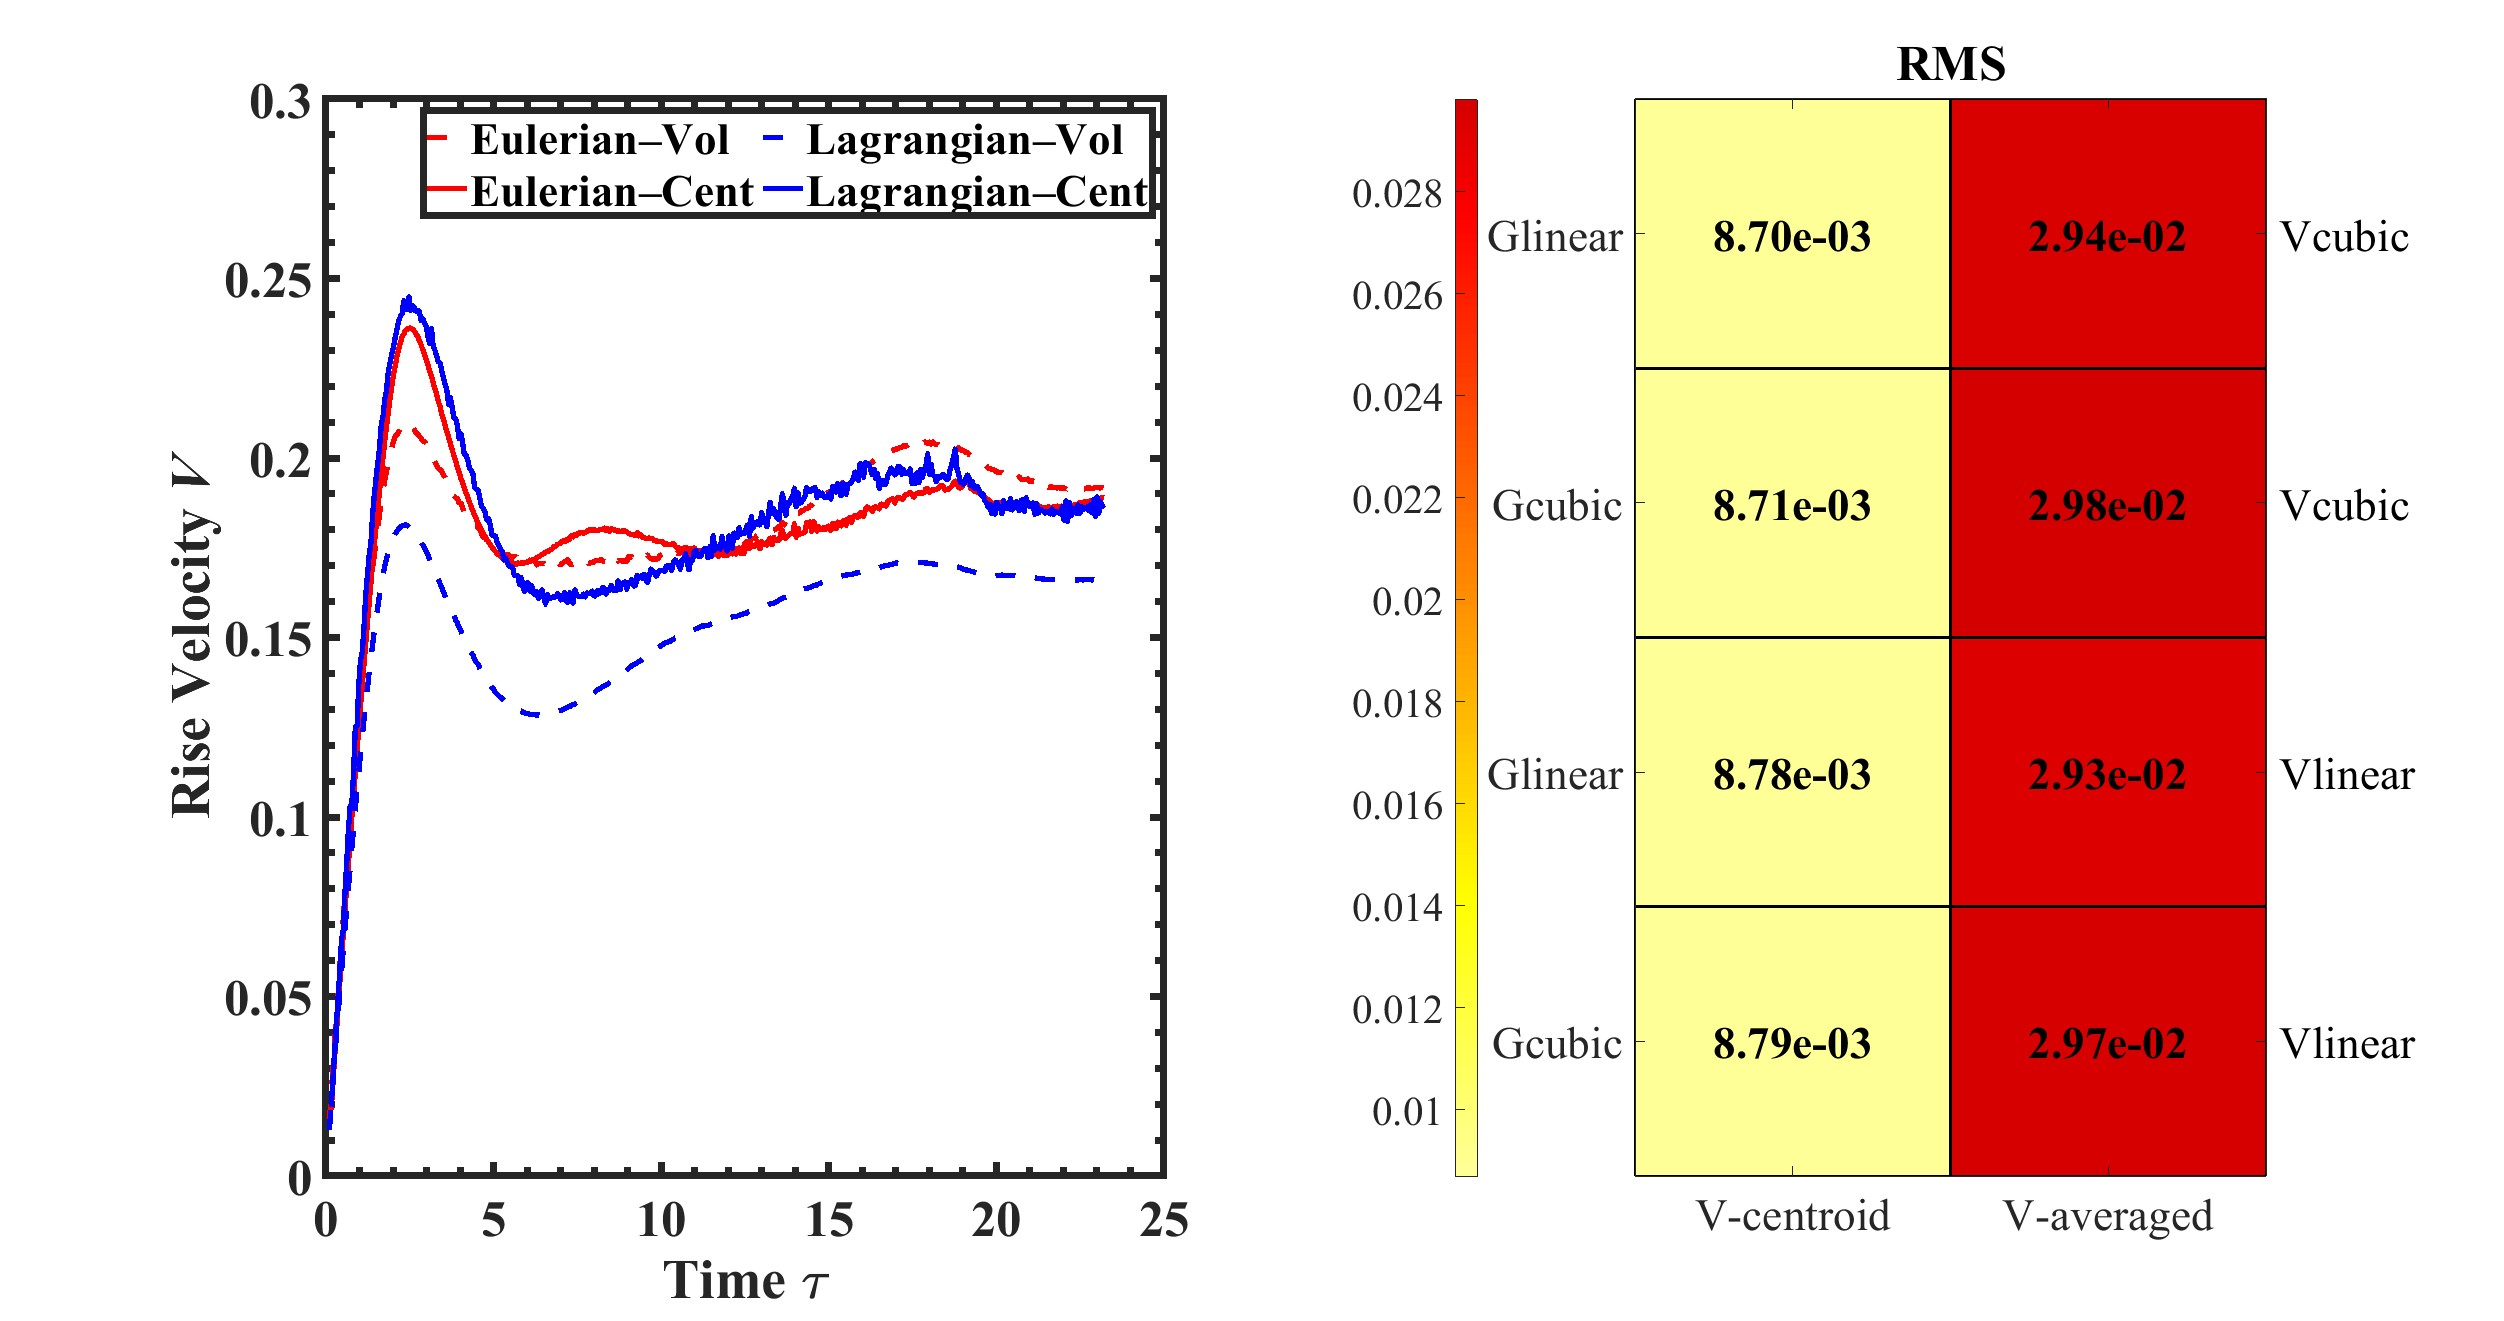
\includegraphics[width=\textwidth]{Fig1a.jpg}
  \caption{%
    Scattered Lagrangian data (Approach~A).
    \textbf{Left:} Temporal evolution of the non-dimensional rise velocity,
    comparing the Eulerian reference (red) with the scattered Lagrangian
    estimate (blue) for the first interpolation case.  Solid lines
    correspond to the centroid-based method; dashed lines to the
    volume-averaged method.
    \textbf{Right:} RMS error heatmap across all four interpolation
    combinations.  Rows indicate the gas fraction interpolation scheme and
    columns distinguish between centroid-based and volume-averaged methods.
    Labels on the right margin identify the velocity interpolation scheme.}
  \label{fig:fig1a}
\end{figure}

% --- Figure 1b: Scattered field profiles ---
\begin{figure}[ht]
  \centering
  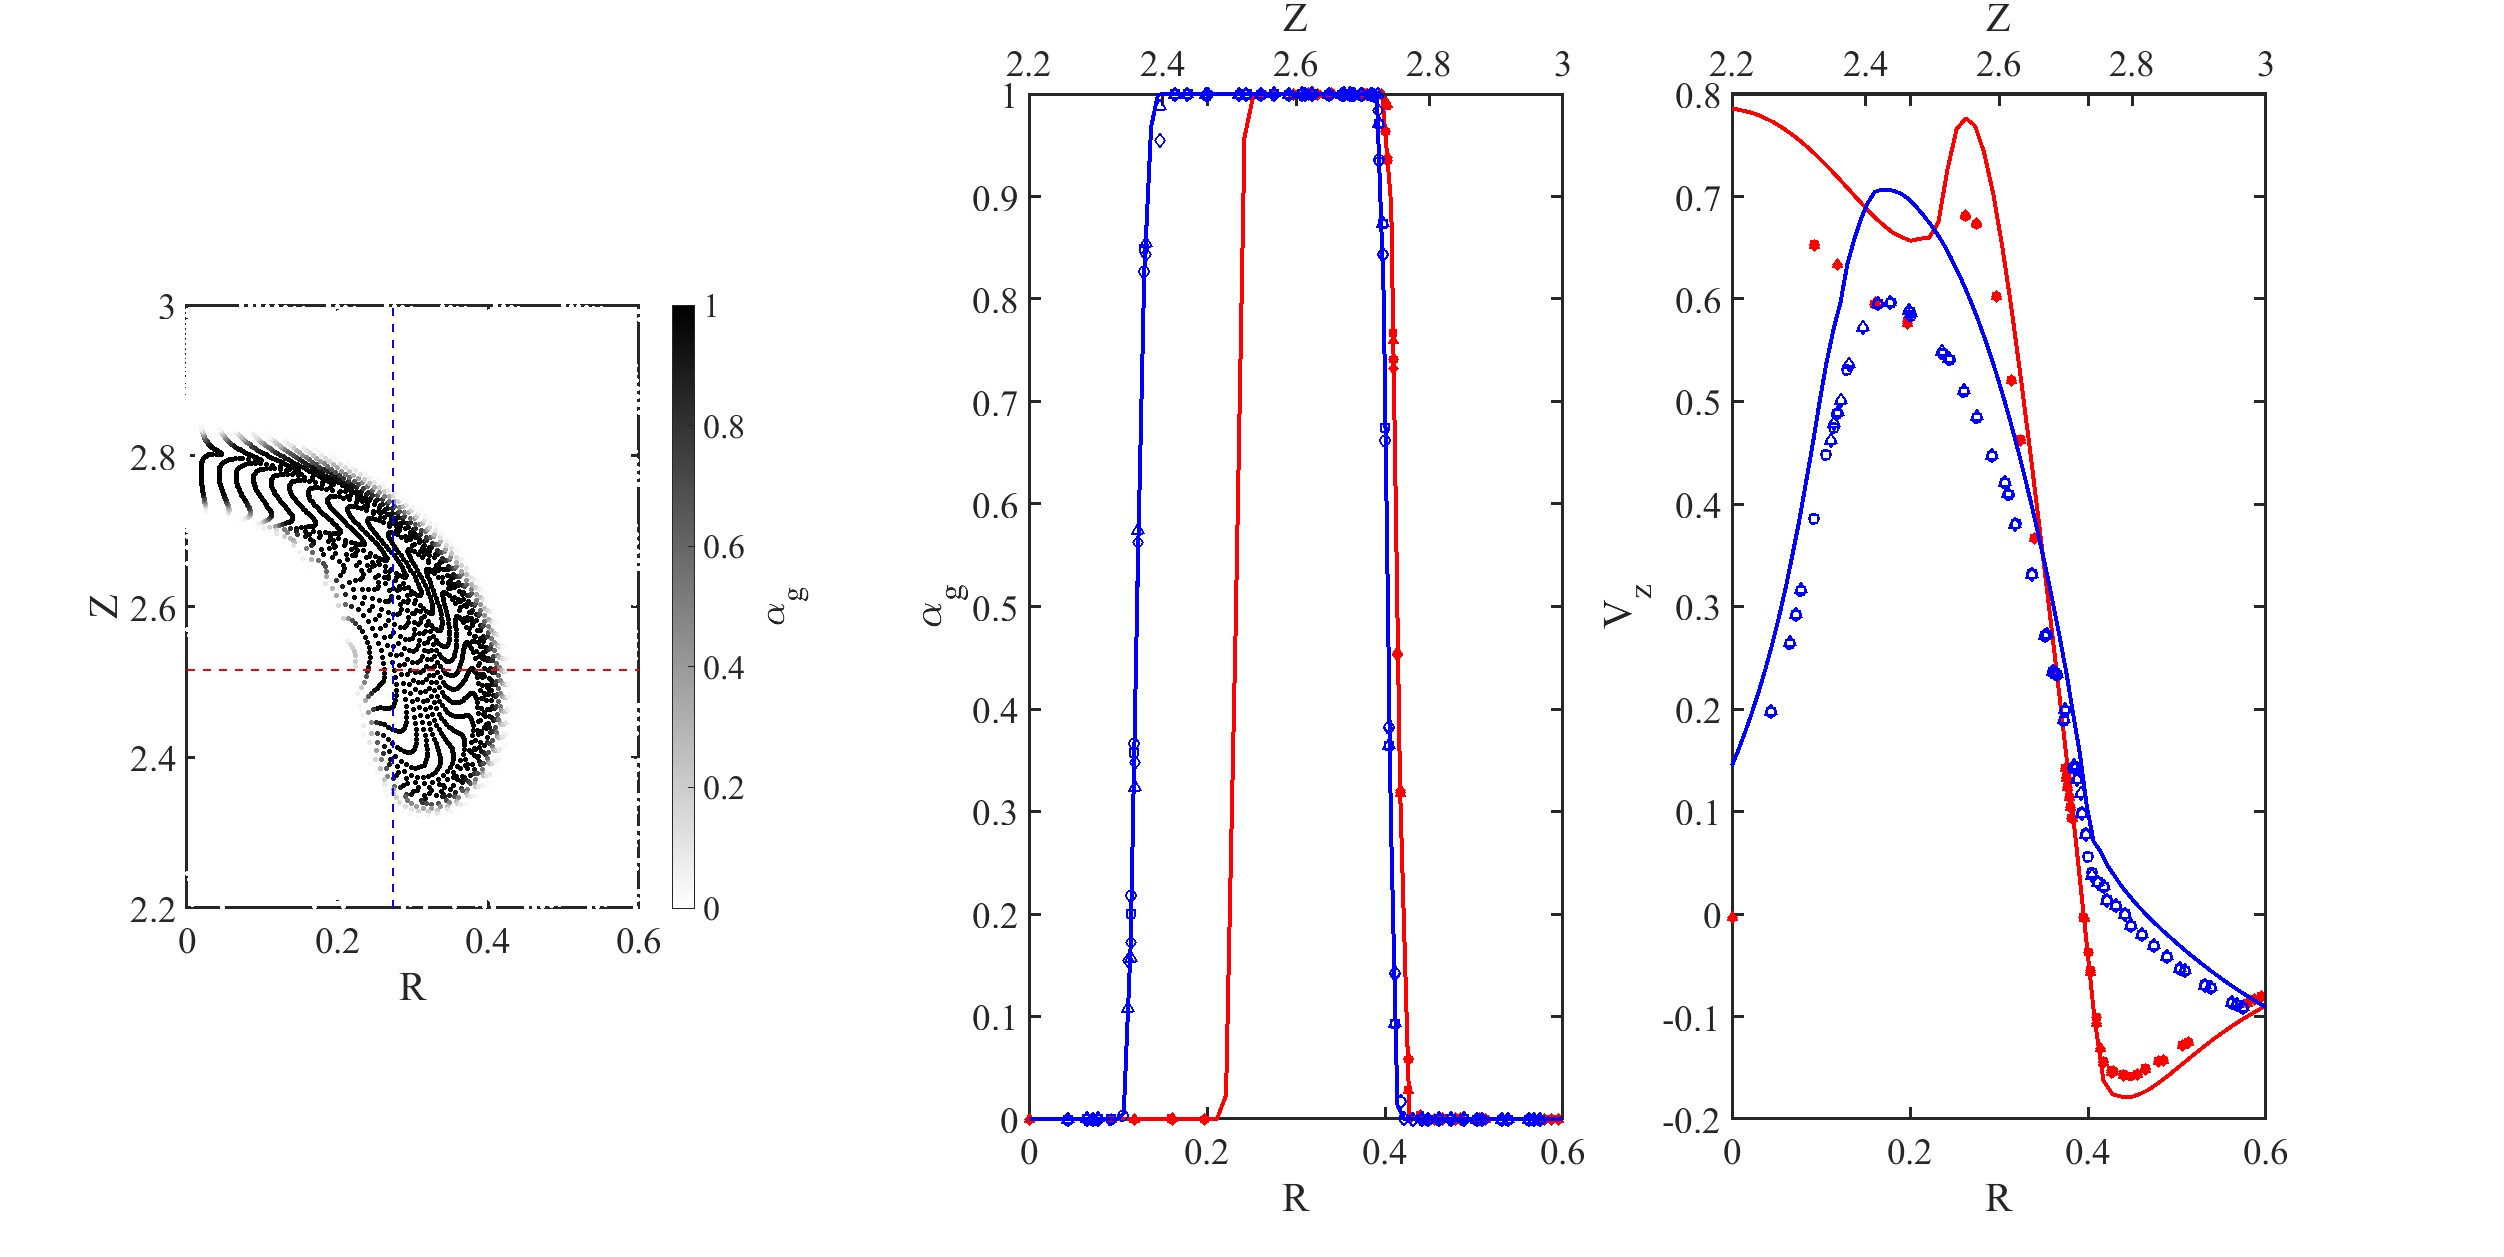
\includegraphics[width=\textwidth]{Fig1b.jpg}
  \caption{%
    Scattered Lagrangian data (Approach~A) at $\tau \approx 6.3$.
    \textbf{Left:} Scatter plot of Lagrangian particle positions coloured by
    the gas volume fraction $\alphag$; dashed lines indicate the horizontal
    (red, $r$-direction) and vertical (blue, $z$-direction) cut-lines.
    \textbf{Middle:} Gas fraction profiles along the two cut-lines:
    Eulerian reference (solid lines) versus scattered Lagrangian values
    (markers) for all four interpolation combinations.
    Red denotes the $r$-direction (bottom axis); blue denotes the
    $z$-direction (top axis).
    \textbf{Right:} Corresponding axial velocity profiles.
    The larger scatter in velocity compared with gas fraction confirms that
    $\Vz$ interpolation is the dominant error source.}
  \label{fig:fig1b}
\end{figure}

% --- Figure 2a: Interpolated rise velocity + RMS heatmap ---
\begin{figure}[ht]
  \centering
  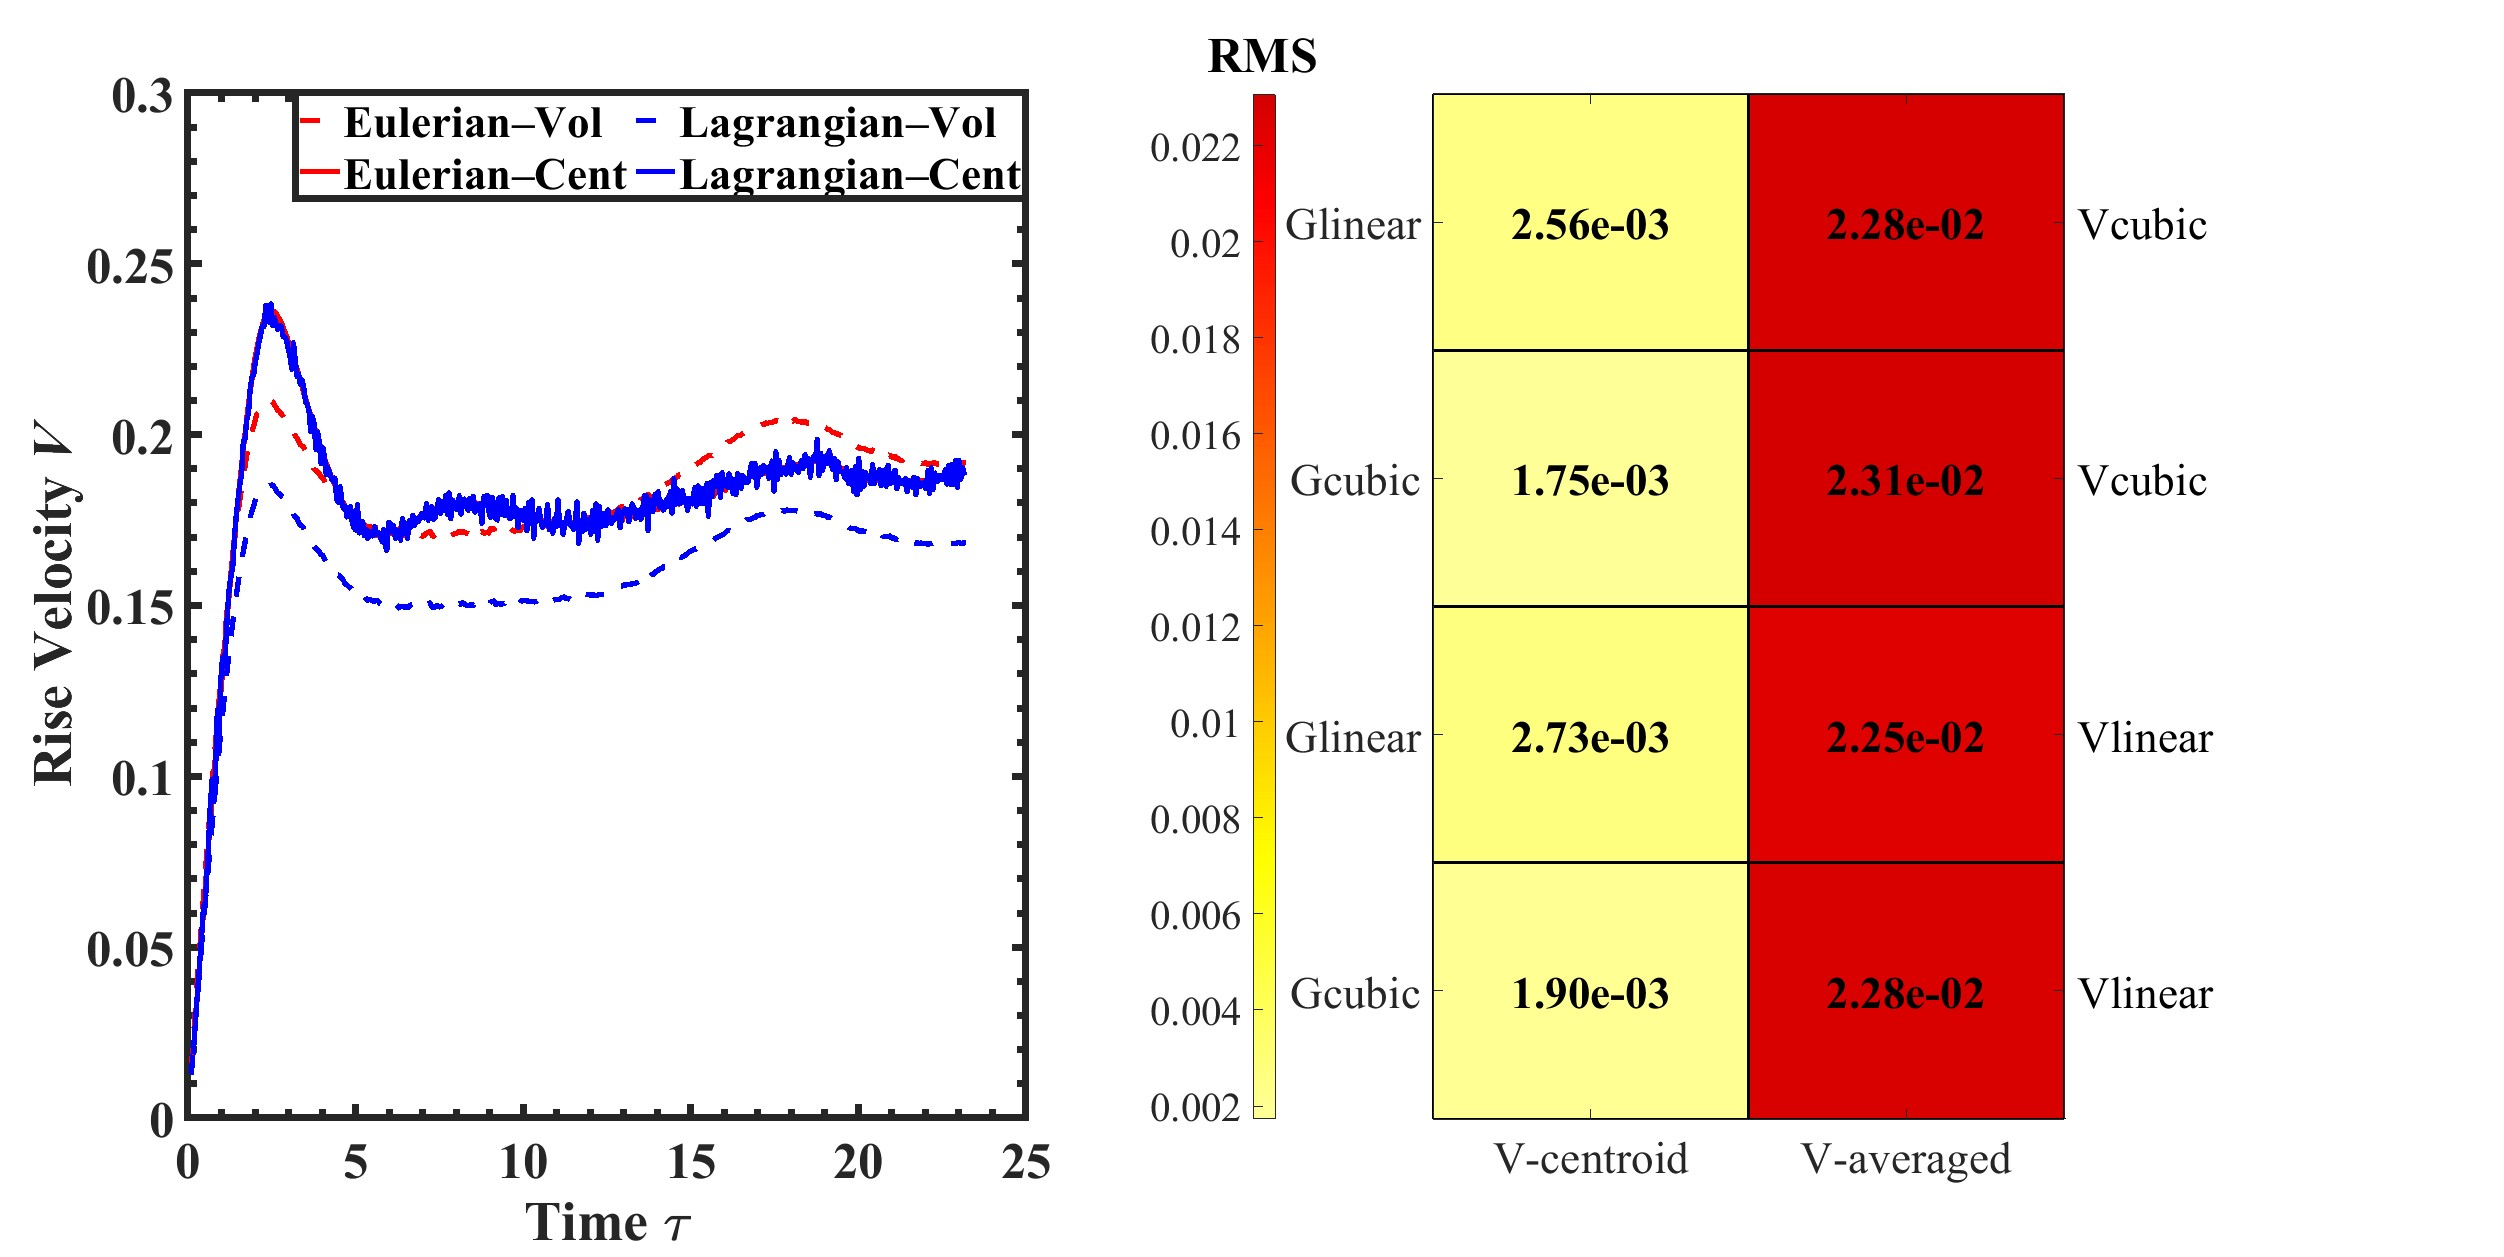
\includegraphics[width=\textwidth]{Fig2a.jpg}
  \caption{%
    Re-interpolated Lagrangian data (Approach~B).
    \textbf{Left:} Temporal evolution of the non-dimensional rise velocity
    after re-interpolation.  The centroid-based Lagrangian estimate (blue
    solid) now nearly overlaps the Eulerian reference (red solid), while the
    volume-averaged estimate (blue dashed) remains offset.
    \textbf{Right:} RMS error heatmap.  Centroid-based errors have decreased
    by a factor of 3--5 compared with \cref{fig:fig1a}; volume-averaged
    errors show only modest improvement.}
  \label{fig:fig2a}
\end{figure}

% --- Figure 2b: Interpolated field profiles ---
\begin{figure}[ht]
  \centering
  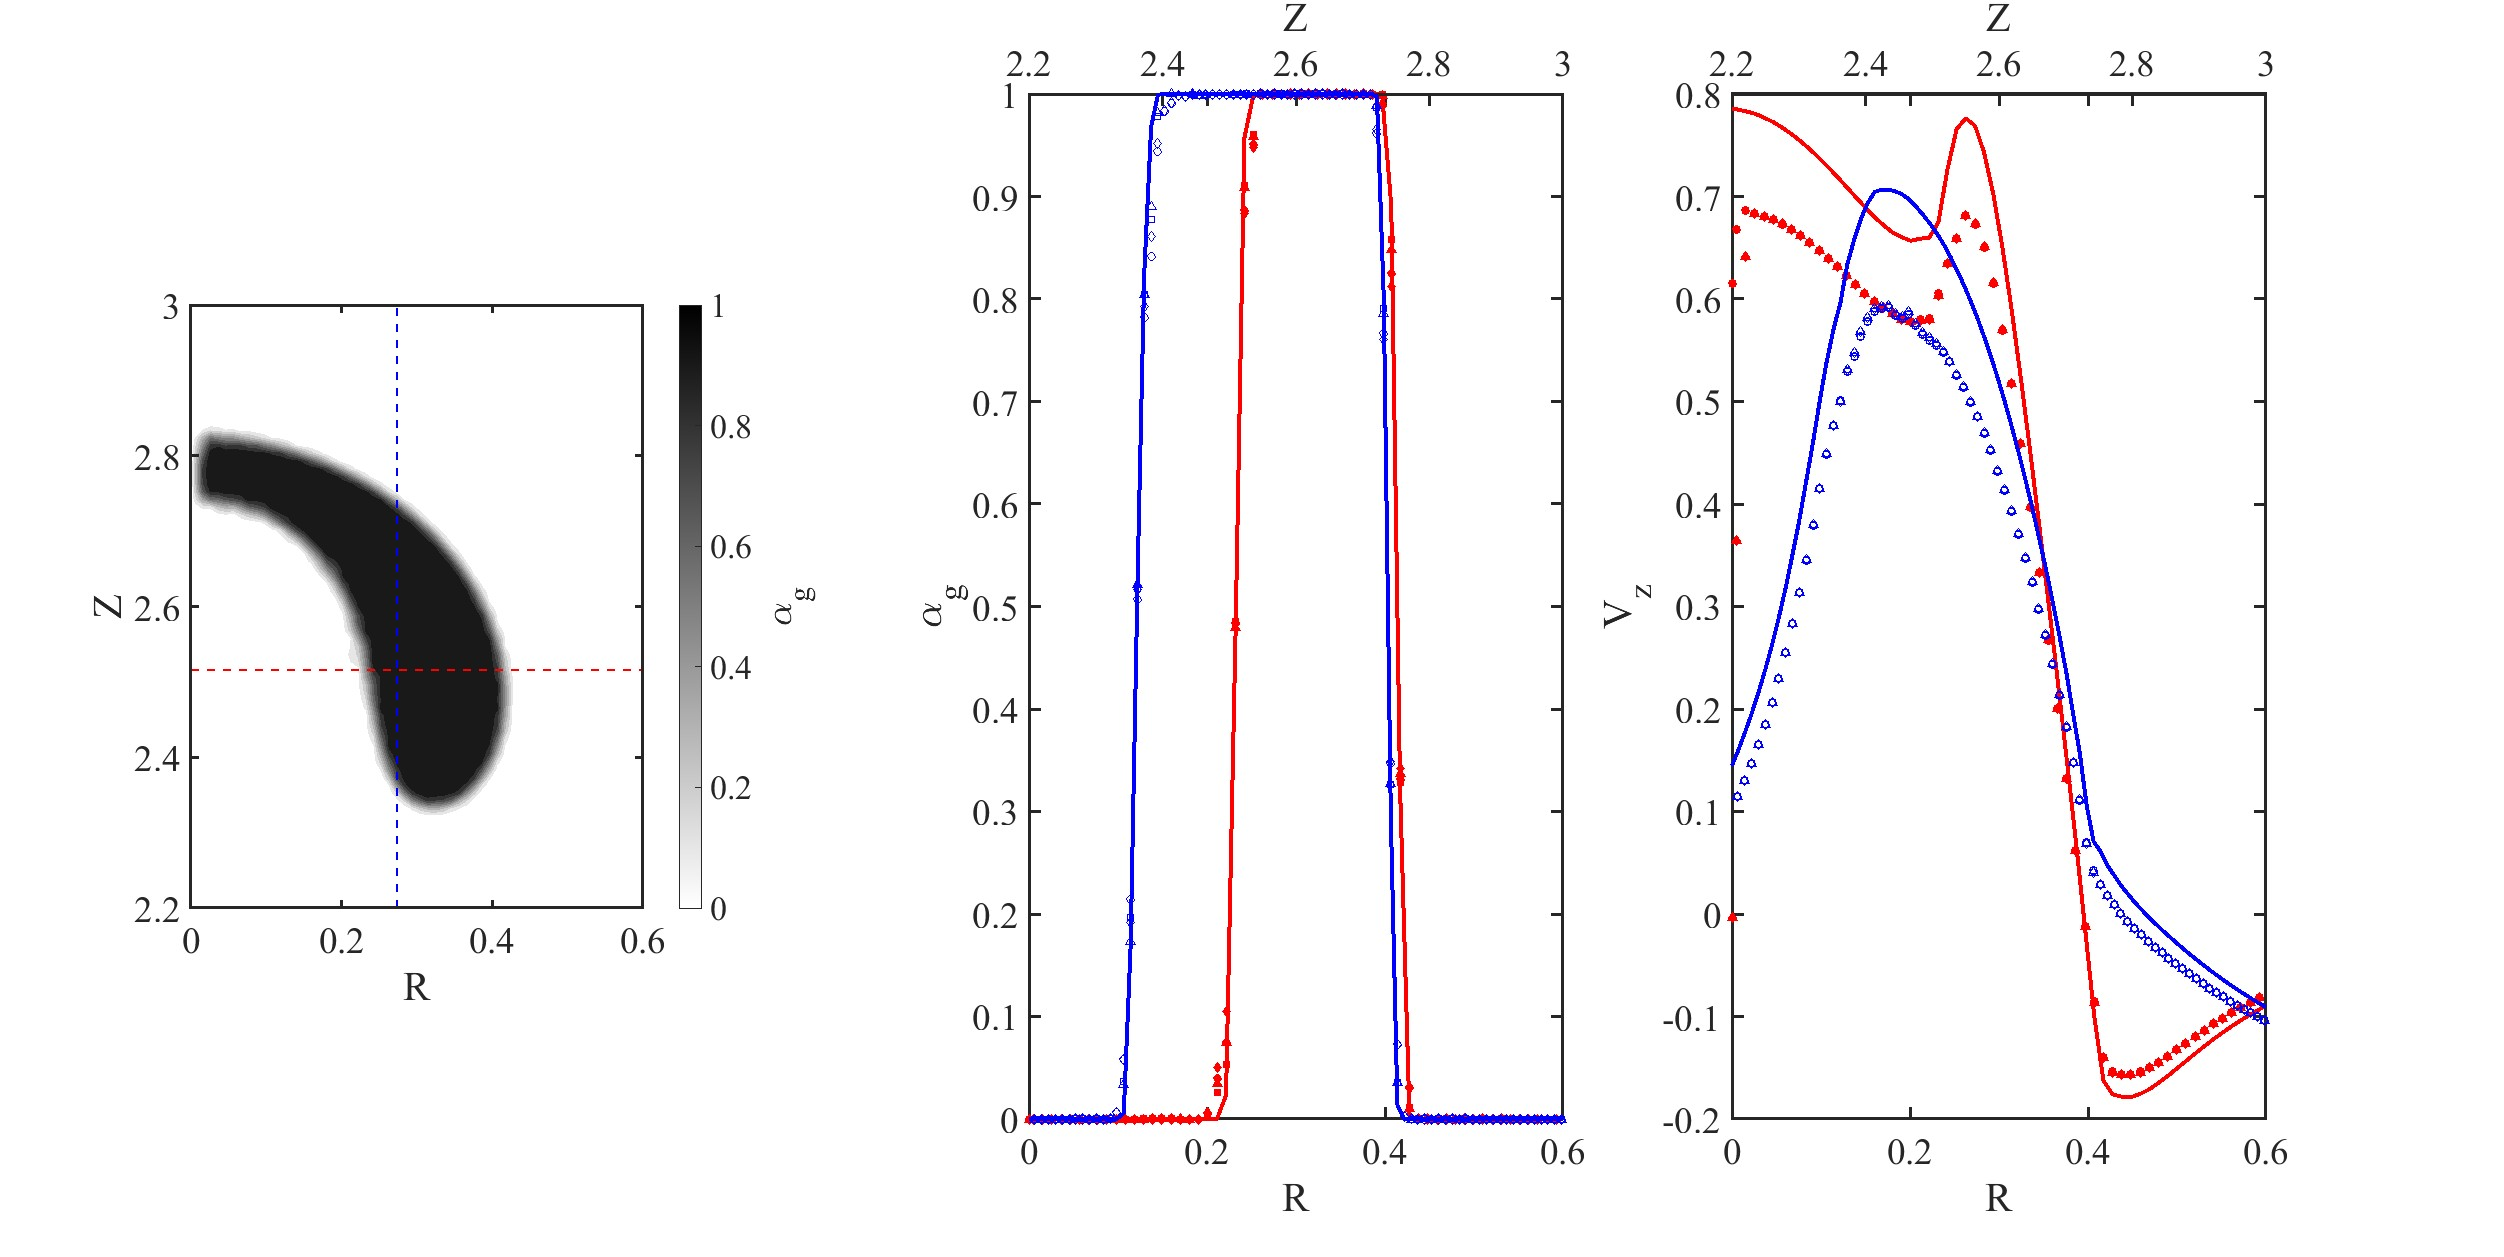
\includegraphics[width=\textwidth]{Fig2b.jpg}
  \caption{%
    Re-interpolated Lagrangian data (Approach~B) at $\tau \approx 6.3$.
    \textbf{Left:} Contour plot of the re-interpolated gas fraction field
    for the first Lagrangian case, with diagnostic cut-lines indicated.
    \textbf{Middle:} Re-interpolated gas fraction profiles along the
    cut-lines, now smooth and closely matching the Eulerian reference.
    \textbf{Right:} Re-interpolated velocity profiles.  While smoother
    than the scattered counterpart (\cref{fig:fig1b}), deviations from the
    Eulerian reference persist, particularly near the bubble boundary.}
  \label{fig:fig2b}
\end{figure}


\end{document}
